\section{B-splines}

\begin{exercise}
    Suppose that $x_0, x_1, x_2$ are distinct, and let $f_i = f(x_i)$, $i = 0, 1, 2$, for some function $f$.
    Show by direct calculation that the recursive formula
    \begin{equation*}
        [x_0, x_1, x_2]f =
        \frac{
            \frac{f_2 - f_1}{x_2 - x_1}
            - \frac{f_1 - f_0}{x_1 - x_0}
        }{x_2 - x_0}
    \end{equation*}
    can be expressed as
    \begin{equation*}
        [x_0, x_1, x_2]f = \sum_{i=0}^{2} \frac{f_i}{\prod_{j \neq i} (x_i - x_j)}.
    \end{equation*}
\end{exercise}

\begin{solution}
    We have
    \begin{align*}
        [x_0, x_1, x_2]f
        &= \frac{
            \frac{f_2 - f_1}{x_2 - x_1}
            - \frac{f_1 - f_0}{x_1 - x_0}
        }{x_2 - x_0}
    \end{align*}
    where we begin by expanding the top fractions.
    \begin{align}
        \frac{f_2 - f_1}{x_2 - x_1} - \frac{f_1 - f_0}{x_1 - x_0}
        &= \frac{f_2}{x_2 - x_1} - f_1 \left( \frac{1}{x_2 - x_1} + \frac{1}{x_1 - x_0} \right) + \frac{f_0}{x_1 - x_0} \nonumber \\
        &= \frac{f_2}{x_2 - x_1} - f_1 \frac{x_1 - x_0 + x_2 - x_1}{(x_2 - x_1)(x_1 - x_0)} + \frac{f_0}{x_1 - x_0} \nonumber \\
        &= \frac{f_2}{x_2 - x_1} - f_1 \frac{x_2 - x_0}{(x_2 - x_1)(x_1 - x_0)} + \frac{f_0}{x_1 - x_0} \nonumber \\
        &= \frac{f_2}{x_2 - x_1} + \frac{f_1(x_2 - x_0)}{(x_1 - x_2)(x_1 - x_0)} + \frac{f_0}{x_1 - x_0} \label{eq:top_fraction}
    \end{align}
    Dividing~\eqref{eq:top_fraction} by $x_2 - x_0$ gives
    \begin{align*}
        [x_0, x_1, x_2]f
        &= \frac{
            \frac{f_2 - f_1}{x_2 - x_1}
            - \frac{f_1 - f_0}{x_1 - x_0}
        }{x_2 - x_0} \\
        &= \frac{f_2}{(x_2 - x_1)(x_2 - x_0)}
        + \frac{f_1}{(x_1 - x_2)(x_1 - x_0)}
        + \frac{f_0}{(x_1 - x_0)(x_2 - x_0)} \\
        &= \frac{f_2}{(x_2 - x_1)(x_2 - x_0)}
        + \frac{f_1}{(x_1 - x_2)(x_1 - x_0)}
        + \frac{f_0}{(x_0 - x_1)(x_0 - x_2)} \\
        &= \sum_{i=0}^{2} \frac{f_i}{\prod_{j \neq i} (x_i - x_j)},
    \end{align*}
    as desired.
\end{solution}

\begin{exercise}
    Show that if $f(x) = 1/x$ and that $x_0, x_1, \ldots, x_k \neq 0$ then
    \begin{equation*}
        [x_0, \ldots, x_k]f = (-1)^k \frac{1}{x_0 x_1 \cdots x_k}.
    \end{equation*}
\end{exercise}

\begin{solution}
    In the base case we have simply
    \begin{equation*}
        [x_0]f = \frac{1}{x_0} = (-1)^0 \frac{1}{x_0}.
    \end{equation*}
    In the case of $x_0 = x_1 = \cdots = x_k$ we have
    \begin{equation*}
        [\underbrace{x_0, x_0, \ldots, x_0}_{k+1}]f = \frac{f^{(k)}(x_0)}{k!} = (-1)^k \frac{1}{x_0^{k+1}} \frac{k!}{k!} = (-1)^k \frac{1}{x_0 x_1 \cdots x_k},
    \end{equation*}
    so mulitplicities are handled correctly.
    For two distinct points $x_0, x_1$ we have
    \begin{equation*}
        [x_0, x_1]f = \frac{f_1 - f_0}{x_1 - x_0} = \frac{1/x_1 - 1/x_0}{x_1 - x_0} = \frac{x_0 - x_1}{x_0 x_1 (x_1 - x_0)} = (-1)^1 \frac{1}{x_0 x_1},
    \end{equation*}
    so the formula holds for $k = 1$.
    Assume that the formula holds for $k = n$, and consider $k = n + 1$.
    We have
    \begin{align*}
        [x_0, \ldots, x_{n+1}]f
        &= \frac{[x_1, \ldots, x_{n+1}]f - [x_0, \ldots, x_{n}]f}{x_{n+1} - x_0} \\
        &= \frac{(-1)^n \frac{1}{x_1 \cdots x_{n+1}} - (-1)^n \frac{1}{x_0 \cdots x_n}}{x_{n+1} - x_0} \\
        &= \frac{
            (-1)^n \frac{1}{x_{n+1}} - (-1)^n \frac{1}{x_0}
        }{
            (x_{n+1} - x_0) x_1 \cdots x_n
        } \\
        &= \frac{
            (-1)^n \frac{x_0 - x_{n+1}}{x_0 x_{n+1}}
        }{
            (x_{n+1} - x_0) x_1 \cdots x_n
        } \\
        &= (-1)^{n+1}\frac{
            x_{n+1} - x_0
        }{
            (x_{n+1} - x_0) x_0 x_1 \cdots x_n x_{n+1}
        } \\
        &= (-1)^{n+1}\frac{1}{x_0 x_1 \cdots x_{n+1}},
    \end{align*}
    proving the formula by induction.
\end{solution}

\begin{exercise}
    Prove the Leibniz rule for divided differences:
    \begin{equation*}
        [x_0, x_1, \ldots, x_k](fg) = \sum_{i=0}^{k} [x_0, \ldots, x_i]f [x_i, \ldots, x_k]g.
    \end{equation*}
    Hint: let $p$ and $q$ be the polynomials of degree $\leq k$ that interpolate $f$ and $g$ respectively at $x_0, x_1, \ldots, x_k$, and express $p$ and $q$ as
    \begin{align*}
        p(x) &= \sum_{i=0}^{k} (x - x_0) \cdots (x - x_{i-1})[x_0, \ldots, x_i]f, \\
        q(x) &= \sum_{j=0}^{k} (x - x_{j+1}) \cdots (x - x_k)[x_j, \ldots, x_k]g.
    \end{align*}
    Now consider the polynomial $pq$.
\end{exercise}

\begin{comment}
\begin{solution}
    Considering the hint, it seems important to consider the definition of divided differences based on the leading coefficient of the interpolating polynomial.
    Let $p$ and $q$ be the polynomials of degree $\leq k$ that interpolate $f$ and $g$ respectively at $x_0, x_1, \ldots, x_k$, and lets assume for now that $x_i \neq x_j$ for $i \neq j$.
    We write $p$ and $q$ as
    \begin{align*}
        p(x) &= \sum_{i=0}^{k} (x - x_0) \cdots (x - x_{i-1})[x_0, \ldots, x_i]f, \\
        q(x) &= \sum_{j=0}^{k} (x - x_{j+1}) \cdots (x - x_k)[x_j, \ldots, x_k]g,
    \end{align*}
    that is, in Newton form, where $q$ is written in reverse order.

    We now consider the polynomial $pq$.
    For brevity, we write $p$ and $q$ as
    \begin{equation*}
        p(x) = \sum_{i = 0}^k \prod_{a = 0}^{i - 1} (x - x_a) [x_0, \ldots, x_i]f,
        \quad
        q(x) = \sum_{j = 0}^k \prod_{b = j + 1}^{k} (x - x_b) [x_j, \ldots, x_k]g.
    \end{equation*}
    Then,
    \begin{align*}
        (p \cdot q)(x)
        &= \left( \sum_{i = 0}^k \prod_{a = 0}^{i - 1} (x - x_a) [x_0, \ldots, x_i]f \right) \left( \sum_{j = 0}^k \prod_{b = j + 1}^{k} (x - x_b) [x_j, \ldots, x_k]g \right) \\
        &= \sum_{i = 0}^k \sum_{j = 0}^k \prod_{a = 0}^{i - 1} (x - x_a) [x_0, \ldots, x_i]f \prod_{b = j + 1}^{k} (x - x_b) [x_j, \ldots, x_k]g \\
        &= \sum_{i = 0}^k \sum_{j = 0}^k [x_0, \ldots, x_i]f [x_j, \ldots, x_k]g \prod_{a = 0}^{i - 1} (x - x_a) \prod_{b = j + 1}^{k} (x - x_b).
    \end{align*}

    What about the unique polynomial of degree $\leq k$ that interpolates $fg$ at $x_0, x_1, \ldots, x_k$?
    We know that the polynomial must be of the form
    \begin{equation*}
        r(x) = \sum_{m = 0}^k [x_0, \ldots, x_m](fg) \prod_{n = 0}^{m - 1} (x - x_n),
    \end{equation*}
    and we know that $r(x)$ must be equal to $(p \cdot q)(x)$ at $x_0, x_1, \ldots, x_k$, as
    \begin{equation*}
        r(x_i) = f_i \cdot g_i = p(x_i) \cdot q(x_i) = (p \cdot q)(x_i),
        \quad i = 0, 1, \ldots, k.
    \end{equation*}

    Consider now a specific $x_\ell \in \{x_0, \ldots, x_k\}$.
    We have
    \begin{align*}
        r(x_\ell)
        &= \sum_{m = 0}^k [x_0, \ldots, x_m](fg) \prod_{n = 0}^{m - 1} (x_\ell - x_n) \\
        &= \sum_{m = 0}^\ell [x_0, \ldots, x_m](fg) \prod_{n = 0}^{m - 1} (x_\ell - x_n) + \sum_{m = \ell + 1}^k [x_0, \ldots, x_m](fg) \prod_{n = 0}^{m - 1} (x_\ell - x_n) \\
        &= \sum_{m = 0}^\ell [x_0, \ldots, x_m](fg) \prod_{n = 0}^{m - 1} (x_\ell - x_n),
    \end{align*}
    where the last equality follows as $\prod_{n = 0}^{m - 1} (x_\ell - x_n) = 0$ for $m > \ell$.
    Considering $p$ and $q$ seperately, we similarly have
    \begin{align*}
        p(x_\ell)
        &= \sum_{i = 0}^k [x_0, \ldots, x_i]f \prod_{a = 0}^{i - 1} (x_\ell - x_a) , \\
        &= \sum_{i = 0}^\ell [x_0, \ldots, x_i]f \prod_{a = 0}^{i - 1} (x_\ell - x_a) ,
    \end{align*}
    and
    \begin{align*}
        q(x_\ell)
        &= \sum_{j = 0}^k [x_j, \ldots, x_k]g \prod_{b = j + 1}^{k} (x_\ell - x_b) , \\
        &= \sum_{j = \ell}^k [x_j, \ldots, x_k]g \prod_{b = j + 1}^{k} (x_\ell - x_b) .
    \end{align*}

    In order to get a better intuition as to how to proceed, let's consider the points $x_0$.
    We have
    \begin{equation*}
        r(x_0) = [x_0](fg) = f_0 g_0
        \quad \text{and} \quad
        p(x_0) = [x_0]f = f_0,
    \end{equation*}
    while $q$ gives us
    \begin{equation*}
        q(x_0) =
        \sum_{j = 0}^k [x_j, \ldots, x_k]g \prod_{b = j + 1}^{k} (x_0 - x_b).
    \end{equation*}
    We already know that $q(x_0) = g_0$, however actually calculating everything seems tricky, likely involving some telescoping sum from the recursive formula.

    Multiplying $p$ and $q$ at $x_\ell$ gives
    \begin{equation*}
        p(x_\ell) \cdot q(x_\ell) = \sum_{i = 0}^\ell \sum_{j = \ell}^k [x_0, \ldots, x_i]f [x_j, \ldots, x_k]g \prod_{a = 0}^{i - 1} (x_\ell - x_a) \prod_{b = j + 1}^{k} (x_\ell - x_b).
    \end{equation*}
    This seems pretty close if you ask me, if you compare with $r(x_\ell)$, however I'm unsure as to how to compute the summations and products.
    The leading power of $x_\ell$ is found $i = \ell = j$, which includes the term
    \begin{equation*}
        \prod_{a=0}^{\ell-1} (x_\ell - x_a) \prod_{b = \ell + 1}^{k} (x_\ell - x_b) = \prod_{\substack{a = 0 \\ a \neq \ell}}^{k} (x_\ell - x_a),
    \end{equation*}
    with the coefficient
    \begin{equation*}
        [x_0, \ldots, x_\ell]f [x_\ell, \ldots, x_k]g.
    \end{equation*}
    Interestingly then, the coefficient of the leading power of $x_\ell$ in $r(x_\ell)$ is the same as the coefficient of the leading power of $x_\ell$ in $p(x_\ell) \cdot q(x_\ell)$.

    \vskip 3em % chktex 41

    Lets consider again the polynomial $pq$, taking it from the top.
    We have
    \begin{align*}
        p(x) &= \sum_{i = 0}^k (x - x_0) \cdots (x - x_{i-1})[x_0, \ldots, x_i]f, \\
        q(x) &= \sum_{j = 0}^k (x - x_{j+1}) \cdots (x - x_k)[x_j, \ldots, x_k]g,
    \end{align*}
    and we wish to show that
    \begin{equation*}
        [x_0, \ldots, x_k](fg) = \sum_{i=0}^{k} [x_0, \ldots, x_i]f [x_i, \ldots, x_k]g.
    \end{equation*}
    We also define the polynomial $r$ as
    \begin{equation*}
        r(x) = \sum_{m = 0}^k (x - x_0) \cdots (x - x_{m-1}) [x_0, \ldots, x_m](fg).
    \end{equation*}
    which interpolates $fg$ at $x_0, x_1, \ldots, x_k$.
    With $k = 0$ we have
    \begin{equation*}
        p(x) = [x_0]f
        \quad \text{and} \quad
        q(x) = [x_0]g,
    \end{equation*}
    showing that
    \begin{equation*}
        [x_0](fg) = f_0 g_0 = [x_0]f [x_0]g.
    \end{equation*}

    For $k = 1$ we have
    \begin{align*}
        p(x) &= [x_0]f + (x - x_0)[x_0, x_1]f \\
        q(x) &= (x - x_1)[x_0, x_1]g + [x_1]g \\
        r(x) &= [x_0](fg) + (x - x_0)[x_0, x_1](fg)
    \end{align*}
    where we at $x_0$ have
    \begin{equation*}
        r(x_0) = [x_0](fg)
    \end{equation*}
    and
    \begin{equation*}
        p(x_0) \cdot q(x_0) = [x_0]f((x_0 - x_1)[x_0, x_1]g + [x_1]g)
    \end{equation*}
    using
    \begin{equation*}
        [x_0, x_1]g = \frac{[x_1]g - [x_0]g}{x_1 - x_0}
    \end{equation*}
    we find
    \begin{align*}
        p(x_0) \cdot q(x_0)
        &= [x_0]f((x_0 - x_1)[x_0, x_1]g + [x_1]g) \\
        &= [x_0]f \left( (x_0 - x_1) \frac{[x_1]g - [x_0]g}{x_1 - x_0} + [x_1]g \right) \\
        &= [x_0]f [x_0]g
    \end{align*}
    and similarly
    \begin{equation*}
        p(x_1) \cdot q(x_1) = [x_1]f [x_1]g.
    \end{equation*}
    For $r(x_1)$ we have
    \begin{align*}
        r(x_1)
        &= [x_0](fg) + (x_1 - x_0)[x_0, x_1](fg) \\
        &= [x_0](fg) + (x_1 - x_0) \frac{[x_1](fg) - [x_0](fg)}{x_1 - x_0} \\
        &= [x_1](fg),
    \end{align*}

    IDEA: Consider the polynomial $pq$.
    Multiply everything out, and remove the terms which include factors $(x - x_i)$ for $i = 0, \ldots, k$.
    Removing these still gives us an interpolating polynomials, however it has a lower degree!!!!
\end{solution}
\end{comment}

\begin{solution}
    As the hint suggests, we consider the polynomials $p$ and $q$ of degree $\leq k$ that interpolate $f$ and $g$ respectively at $x_0, x_1, \ldots, x_k$, expressed as
    \begin{align*}
        p(x) &= \sum_{i=0}^{k} (x - x_0) \cdots (x - x_{i-1})[x_0, \ldots, x_i]f, \\
        q(x) &= \sum_{j=0}^{k} (x - x_{j+1}) \cdots (x - x_k)[x_j, \ldots, x_k]g.
    \end{align*}
    In addition, let $r$ be the polynomial of degree $\leq k$ that interpolates $fg$ at $x_0, x_1, \ldots, x_k$, expressed as
    \begin{equation*}
        r(x) = \sum_{m=0}^{k} (x - x_0) \cdots (x - x_{m-1})[x_0, \ldots, x_m](fg).
    \end{equation*}

    We now consider the polynomial $pq$.
    In order to illustrate the idea, let $k = 1$ for now.
    We have
    \begin{align*}
        p(x) &= [x_0]f + (x - x_0)[x_0, x_1]f, \\
        q(x) &= (x - x_1)[x_0, x_1]g + [x_1]g.
    \end{align*}
    The polynomial $pq$ is then
    \begin{multline*}
        pq(x)
        = [x_0]f [x_1]g
        + (x - x_0)[x_0, x_1]f [x_1]g
        + (x - x_1)[x_0]f [x_0, x_1]g \\
        + (x - x_0)(x - x_1)[x_0, x_1]f [x_0, x_1]g.
    \end{multline*}
    We can see that the polynomial $pq$ is of degree $\leq 2$ and interpolates $fg$ at $x_0$ and $x_1$.
    However, note that the rightmost term is zero at both the interpolation points, so removing it still gives us an interpolating polynomial, now of degree $\leq 1$.
    It is therefore the unique interpolating polynomial, of the form
    \begin{equation*}
        \overline{pq}(x)
        = [x_0]f [x_1]g
        + (x - x_0)[x_0, x_1]f [x_1]g
        + (x - x_1)[x_0]f [x_0, x_1]g.
    \end{equation*}
    The leading coefficient of $\overline{pq}$ is then
    \begin{equation*}
        \text{l.c.}(\overline{pq}) = [x_0, x_1]f [x_1]g + [x_0]f [x_0, x_1]g.
    \end{equation*}

    Now, we consider the polynomial $r$.
    We have
    \begin{equation*}
        r(x) = [x_0](fg) + (x - x_0)[x_0, x_1](fg),
    \end{equation*}
    which interpolates $fg$ at $x_0, x_1$.
    Due to the uniqueness of the interpolating polynomial, we must have $r = \overline{pq}$.
    As we can easily see, the leading coefficient of $r$ is
    \begin{equation*}
        \text{l.c.}(r) = [x_0, x_1](fg).
    \end{equation*}
    As the polynomials are the same, the leading coefficients must be the same, so we have
    \begin{equation*}
        [x_0, x_1](fg) = [x_0, x_1]f [x_1]g + [x_0]f [x_0, x_1]g,
    \end{equation*}
    proving the case when $k = 1$.

    We now consider the general case.
    The polynomial $pq$ is now of the form
    \begin{equation*}
        pq(x) = \sum_{i=0}^{k} \sum_{j=0}^{k} [x_0, \ldots, x_i]f [x_j, \ldots, x_k]g \prod_{a=0}^{i-1} (x - x_a) \prod_{b=j+1}^{k} (x - x_b).
    \end{equation*}
    When $j \leq i - 1$, the products on the right side will be zero at $x_0, x_1, \ldots, x_k$, so we can safely remove these terms while still having an interpolating polynomial.
    This gives us $\overline{pq}$, of the form
    \begin{align*}
        \overline{pq}(x) = \sum_{i=0}^{k} \sum_{j=i}^{k} [x_0, \ldots, x_i]f [x_j, \ldots, x_k]g \prod_{a=0}^{i-1} (x - x_a) \prod_{b=j+1}^{k} (x - x_b),
    \end{align*}
    which interpolates $fg$ at $x_0, x_1, \ldots, x_k$ and has degree $\leq k$.
    The leading coefficient of $\overline{pq}$ is found when $i = j$, as it includes the term
    \begin{equation*}
        \prod_{a=0}^{i-1} (x - x_a) \prod_{b=i+1}^{k} (x - x_b) = \prod_{\substack{a=0 \\ a \neq i}}^{k} (x - x_a),
    \end{equation*}
    with the leading coefficient
    \begin{equation*}
        \text{l.c.}(\overline{pq}) = \sum_{i = 0}^{k} [x_0, \ldots, x_i]f [x_i, \ldots, x_k]g.
    \end{equation*}
    From $r$ we can again read the leading coefficient simply as $[x_0, \ldots, x_k](fg)$, proving Leibniz' rule.
\end{solution}

\begin{exercise}
    Use the recursion formula (Theorem~3.4) to show that
    \begin{enumerate}[
    label=\alph*) % chktex 9 % tex-fmt: skip
            ] % chktex 10
        \item $B[0, 0, 0, 1](x) = (1 - x)^2 B[0, 1](x)$,
        \item $B[0, 0, 1, 2](x) = x(2 - 3x/2)B[0, 1](x) + \frac{1}{2}(2 - x)^2B[1, 2](x)$,
        \item $B[0, 1, 1, 2](x) = x^2B[0, 1](x) + (2 - x)^2B[1, 2](x)$.
    \end{enumerate}
\end{exercise}

\begin{solution}
    The recursion formula states that for $d \geq 1$,
    \begin{equation*}
        B_{i, d}(x)
        = \frac{x - t_i}{t_{i+d} - t_i} B_{i, d-1}(x)
        + \frac{t_{i+d+1} - x}{t_{i+d+1} - t_{i+1}} B_{i+1, d-1}(x).
    \end{equation*}
    I'm not entirely sure which knots the $B$-splines are defined on, however I guess the exercise is to relate these ones to the cardinal $B$-splines.

    \begin{enumerate}[
    label=\alph*) % chktex 9 % tex-fmt: skip
            ] % chktex 10
        \item In this case we have $t_i = t_d$, meaning that the first term in the recursion formula is zero.
            We then have
            \begin{align*}
                B[0, 0, 0, 1](x)
                = 0 + \frac{1 - x}{1 - 0} B[0, 0, 1](x).
            \end{align*}
            Recursing on $B[0, 0, 1](x)$, again the first term is zero, so we have
            \begin{equation*}
                (1 - x)B[0, 0, 1](x)
                = (1-x) \frac{1 - x}{1 - 0} B[0, 1](x)
                = (1 - x)^2 B[0, 1](x).
            \end{equation*}

        \item Next, we have
            \begin{gather*}
                B[0, 0, 1, 2](x)
                = \frac{x - 0}{1 - 0} B[0, 0, 1](x)
                + \frac{2 - x}{2 - 0} B[0, 1, 2](x) \\
                = x (1 - x) B[0, 1](x)
                + \frac{2 - x}{2} \left(
                    x B[0, 1](x)
                    + (2 - x) B[1, 2](x)
                \right) \\
                = x \left( 1 - x + \frac{2 - x}{2} \right) B[0, 1](x)
                + \frac{1}{2}(2 - x)^2 B[1, 2](x) \\
                = x \left( 2 - \frac{3}{2}x \right) B[0, 1](x)
                + \frac{1}{2}(2 - x)^2 B[1, 2](x).
            \end{gather*}

        \item Finally, for the last expression we have
            \begin{equation*}
                B[0, 1, 1, 2](x)
                = \frac{x - 0}{1 - 0} B[0, 1, 1](x)
                + \frac{2 - x}{2 - 1} B[1, 1, 2](x).
            \end{equation*}
            Considering the two terms separately, we have
            \begin{equation*}
                B[0, 1, 1](x)
                = x B[0, 1](x)
            \end{equation*}
            as the second term vanishes, and
            \begin{equation*}
                B[1, 1, 2](x)
                = \frac{2 - x}{2 - 1} B[1, 2](x)
                = (2 -x)^2 B[1, 2](x),
            \end{equation*}
            where the first term vanishes.
            Combining these, we find
            \begin{equation*}
                B[0, 1, 1, 2](x)
                = x^2 B[0, 1](x) + (2 - x)^2 B[1, 2](x),
            \end{equation*}
            as desired.
    \end{enumerate}
\end{solution}

\begin{exercise}
    a) Prove Theorem~3.5, and b) use it to show that for distinct knots, % chktex 10 % tex-fmt: skip
    \begin{equation*}
        B_{i, 2}(t_{i+1}) = \frac{t_{i+1} - t_i}{t_{i+2} - t_i},
        \quad
        B_{i, 2}(t_{i+2}) = \frac{t_{i+3} - t_{i+2}}{t_{i+3} - t_{i+1}}.
    \end{equation*}
\end{exercise}

\begin{solution}
    Theorem~3.5 states that for any $j = i, i + 1, \ldots , i + d + 1$,
    \begin{equation*}
        B[t_i, \ldots, t_{i+d+1}](t_j) =
        B[t_i, \ldots, t_{j-1}, t_{j+1}, \ldots, t_{i+d+1}](t_j),
    \end{equation*}
    that is, the spline with the knot $t_j$ removed.

    Let
    \begin{equation*}
        f(x) = (\cdot - x)
        \quad \text{and} \quad
        g(x) = (\cdot - x)_+^{d-1},
    \end{equation*}
    as then
    \begin{equation*}
        \begin{split}
            B_{i,d}(x) &= (t_{i+d+1} - t_i) [t_i, \ldots, t_{i+d+1}](\cdot - x)_+^d \\
            &= (t_{i+d+1} - t_i) [t_i, \ldots, t_{i+d+1}](fg).
        \end{split}
    \end{equation*}
    Dropping the initial coefficient $(t_{i+d+1} - t_i)$ for now, we have by Leibniz' rule
    \begin{align*}
        [t_i, \ldots, t_{i+d+1}](fg)
        &= [t_j, t_i, \ldots, \hat{t}_j, \ldots, t_{i+d+1}](fg) \\
        &= [t_j]f [t_j, t_i, \ldots, \hat{t}_j, \ldots, t_{i+d+1}](g) \\
        &\quad + [t_j, t_i]f [t_i, \ldots, \hat{t}_j, \ldots, t_{i+d+1}](g) \\
        &\quad + [t_j, t_i, t_{i+1}]f [t_{i+1}, \ldots, \hat{t}_j, \ldots, t_{i+d+1}](g) \\
        &\quad + \cdots,
    \end{align*}
    where the hat denotes the omitted knot.
    As $f$ is linear, we have
    \begin{equation*}
        [\underbrace{t_j, t_i, \ldots, t_k}_{\geq 3}]f = 0
        \quad \text{and} \quad
        [t_j, t_i]f = 1.
    \end{equation*}
    We then have
    \begin{equation*}
        \begin{split}
            [t_i, \ldots, t_{i+d+1}](fg) &= f(t_j) [t_j, t_i, \ldots, \hat{t}_j, \ldots, t_{i+d+1}](g) \\
            &\quad + [t_i, \ldots, \hat{t}_j, \ldots, t_{i+d+1}](g) \\
            &= (t_j - x) [t_j, t_i, \ldots, \hat{t}_j, \ldots, t_{i+d+1}](g) \\
            &\quad + [t_i, \ldots, \hat{t}_j, \ldots, t_{i+d+1}](g).
        \end{split}
    \end{equation*}
    At $x = t_j$, we thus have, instering back the coefficient,
    \begin{equation*}
        B[t_i, \ldots, t_{i+d+1}](t_j) =
        B[t_i, \ldots, \hat{t}_j, \ldots, t_{i+d+1}](t_j),
    \end{equation*}
    as we wanted to show.

    For the second part, we have
    \begin{align*}
        B_{i, 2}(t_{i+1}) &= B[t_i, t_{i+1}, t_{i+2}, t_{i+3}](t_{i+1}) = B[t_i, t_{i+2}, t_{i+3}](t_{i+1}) \\
        &= \frac{t_{i+1} - t_i}{t_{i+2} - t_i} B[t_i, t_{i+2}](t_{i+1}) + \frac{t_{i+3} - t_{i+1}}{t_{i+3} - t_{i+2}} B[t_{i+2}, t_{i+3}](t_{i+1}) \\
        &= \frac{t_{i+1} - t_i}{t_{i+2} - t_i}
    \end{align*}
    Here, we've used that $B[a, b](x) = 0$ for $x \notin [a, b)$, and $B[a, b](x) = 1$ for $x \in [a, b)$. % chktex 9
    For the second expression we similarly have
    \begin{align*}
        B_{i, 2}(t_{i+2}) &= B[t_i, t_{i+1}, t_{i+2}, t_{i+3}](t_{i+2}) = B[t_i, t_{i+1}, t_{i+3}](t_{i+2}) \\
        &= \frac{t_{i+2} - t_i}{t_{i+3} - t_i} B[t_i, t_{i+1}](t_{i+2}) + \frac{t_{i+3} - t_{i+2}}{t_{i+3} - t_{i+1}} B[t_{i+1}, t_{i+3}](t_{i+2}) \\
        &= \frac{t_{i+3} - t_{i+2}}{t_{i+3} - t_{i+1}}.
    \end{align*}
\end{solution}

\begin{exercise}
    Show that
    \begin{align*}
        B[\underbrace{a, \ldots, a}_{d+1}, b](x) &= \left(\frac{b - x}{b - a}\right)^d B[a, b](x), \\
        B[a, \underbrace{b, \ldots, b}_{d+1}](x) &= \left(\frac{x - a}{b - a}\right)^d B[a, b](x).
    \end{align*}
    Use this to show that
    \begin{equation*}
        B[a, \underbrace{b, \ldots, b}_{d}, c](x) = \left(\frac{x - a}{b - a}\right)^d B[a, b](x) + \left(\frac{c - x}{c - b}\right)^d B[b, c](x).
    \end{equation*}
    Show that this B-spline is continuous on $\mathbb{R}$.
\end{exercise}

\begin{solution}
    We begin by showing the first two expressions.
    Note that when $t_i = t_d$, then
    \begin{equation*}
        [t_i, \ldots, t_d](\cdot - x)_+^{d-1} = 0 \quad \text{for } x \neq t_i,
    \end{equation*}
    and when we additionally define the term to be zero when $x = t_i$, we have
    \begin{equation*}
        B[\underbrace{a, \ldots, a}_{d+1}, b](x) = \frac{b - x}{b - a} B[\underbrace{a, \ldots, a}_{d}, b](x) = \cdots =
        \left(\frac{b - x}{b - a}\right)^d B[a, b](x).
    \end{equation*}
    Similarly, we find that
    \begin{equation*}
        B[a, \underbrace{b, \ldots, b}_{d+1}](x) = \left(\frac{x - a}{b - a}\right)^d B[a, b](x).
    \end{equation*}
    Next, we then have by the recursive formula
    \begin{align*}
        B[a, \underbrace{b, \ldots, b}_{d}, c](x)
        &= \frac{x - a}{b - a} B[a, \underbrace{b, \ldots, b}_{d}](x) + \frac{c - x}{c - b} B[\underbrace{b, \ldots, b}_{d}, c](x) \\
        &= \frac{x - a}{b - a} \left( \frac{x - a}{b - a} \right)^{d-1} B[a, b](x) + \frac{c - x}{c - b} \left( \frac{c - x}{c - b} \right)^{d-1} B[b, c](x) \\
        &= \left(\frac{x - a}{b - a}\right)^{d} B[a, b](x) + \left(\frac{c - x}{c - b}\right)^{d} B[b, c](x).
    \end{align*}

    Using again that
    \begin{equation*}
        B[a, b](x) =
        \begin{cases}
            0, & x \notin [a, b), \\ % chktex 9
            1, & x \in [a, b), % chktex 9
        \end{cases}
    \end{equation*}
    we can rewrite the spline as
    \begin{equation*}
        B[a, \underbrace{b, \ldots, b}_{d}, c](x) =
        \begin{cases}
            \left( \frac{x - a}{b - a} \right)^d & x \in [a, b), \\ % chktex 9
            \left( \frac{c - x}{c - b} \right)^{d} & x \in [b, c), \\ % chktex 9
            0 & \text{otherwise}.
        \end{cases}
    \end{equation*}
    At the knot $b$, the spline is continuous, as
    \begin{equation*}
        \frac{b - a}{b - a} = 1 = \frac{c - b}{c - b},
    \end{equation*}
    while they are both zero at $x = a$ and $x = c$ respectively.
\end{solution}

\begin{exercise}
    Show that
    \begin{equation*}
        B_{i, d}(x) = (-1)^{d+1} (t_{i+d+1} - t_i) [t_i, t_{i+1}, \ldots, t_{i+d+1}] (x - \cdot)_+^{d},
        \quad x \in \mathbb{R}.
    \end{equation*}
    Hint: Use the fact that
    \begin{equation*}
        (t - x)_{+}^{d} - (-1)^{d+1} (x - t)_{+}^{d} = (t - x)^d.
    \end{equation*}
    Use this to show that for distinct knots,
    \begin{equation*}
        B_{i,d}(x) = (t_{i+d+1} - t_i) \sum_{j = i}^{i + d + 1} \frac{(x - t_j)_+^d}{\prod_{\substack{k = i \\ k \neq j}}^{i + d + 1} (t_k - t_j)}.
    \end{equation*}
\end{exercise}

\begin{solution}
    A reasonable place to start baced on the hint seems to note that
    \begin{equation*}
        (t - x)_+^d = (-1)^{d+1} (x - t)_+^d - (t - x)^d.
    \end{equation*}
    Then, if we can show that
    \begin{equation*}
        [t_i, t_{i+1}, \ldots, t_{i+d+1}] (\cdot - x)^d = 0
    \end{equation*}
    we are practically done with the first part.
    As $(t - x)^d$ is a polynomial of degree $d$, and we have $d + 1$ knots, the term vanishes.

    We then have
    \begin{align*}
        B_{i, d}(x)
        &= (t_{i+d+1} - t_i) [t_i, t_{i+1}, \ldots, t_{i+d+1}] (\cdot - x)_+^{d} \\
        &= (t_{i+d+1} - t_i) [t_i, t_{i+1}, \ldots, t_{i+d+1}] \left(
            (-1)^{d+1}(x - \cdot)_+^{d} - (t_{i+d+1} - x)^d
        \right) \\
        &= (-1)^{d+1} (t_{i+d+1} - t_i) [t_i, t_{i+1}, \ldots, t_{i+d+1}] (x - \cdot)_+^{d}
    \end{align*}
    as desired.

    We already know by the forward difference formula that we can write
    \begin{equation*}
        B_{i, d}(x)
        = (t_{i+d+1} - t_i) \sum_{j = 1}^{i + d + 1} \frac{
            (t_j - x)_+^d
        }{
            \prod_{\substack{k = i \\ k \neq j}}^{i + d + 1} (t_j - t_k)
        }.
    \end{equation*}
    We can rewrite the denominator as
    \begin{equation*}
        \prod_{\substack{k = i \\ k \neq j}}^{i + d + 1} (t_j - t_k)
        = \prod_{\substack{k = 1 \\ k \neq j}}^{i + d + 1} (-1)(t_k - t_j)
        = (-1)^{d+1} \prod_{\substack{k = 1 \\ k \neq j}}^{i + d + 1} (t_k - t_j).
    \end{equation*}
    Using the forward difference formula on $(-1)^{d+1} (x - t)_+^d$ we then find
    \begin{align*}
        B_{i, d}(x)
        &= (t_{i+d+1} - t_i) (-1)^{d+1} \sum_{j = 1}^{i + d + 1} \frac{
            (x - t_j)_+^d
        }{
            \prod_{\substack{k = i \\ k \neq j}}^{i + d + 1} (t_j - t_k)
        } \\
        &= (t_{i+d+1} - t_i) (-1)^{d+1} \sum_{j = 1}^{i + d + 1} \frac{
            (x - t_j)_+^d
        }{
            (-1)^{d+1} \prod_{\substack{k = i \\ k \neq j}}^{i + d + 1} (t_k - t_j)
        } \\
        &= (t_{i+d+1} - t_i) \sum_{j = 1}^{i + d + 1} \frac{
            (x - t_j)_+^d
        }{
            \prod_{\substack{k = i \\ k \neq j}}^{i + d + 1} (t_k - t_j)
        },
    \end{align*}
    as desired.
\end{solution}

\begin{exercise}
    Use the recursion formula to show that (for $d \geq 1$)
    \begin{equation*}
        \sum_{i = 1}^{n} B_{i, d}(x) = 1,
        \quad x \in [t_{d+1}, t_{n+1}].
    \end{equation*}
\end{exercise}

\begin{solution}
    We have
    \begin{align*}
        \sum_{i = 1}^{n} B_{i, d}(x)
        &= \sum_{i = 1}^{n} \left(
            \frac{x - t_i}{t_{i + d} - t_i} B_{i, d-1}(x)
            + \frac{t_{i + d + 1} - x}{t_{i + d + 1} - t_{i + 1}} B_{i + 1, d-1}(x)
        \right) \\
        &= \sum_{i = 1}^n \frac{x - t_i}{t_{i + d} - t_i} B_{i, d-1}(x)
        + \sum_{i = 1}^{n} \frac{t_{i + d + 1} - x}{t_{i + d + 1} - t_{i + 1}} B_{i + 1, d-1}(x) \\
        &= \sum_{i = 1}^n \frac{x - t_i}{t_{i + d} - t_i} B_{i, d-1}(x)
        + \sum_{i = 2}^{n + 1} \frac{t_{i + d } - x}{t_{i + d} - t_{i}} B_{i, d-1}(x) \\
        &= \frac{x - t_1}{t_{1 + d} - t_1} B_{1, d-1}(x)
        + \sum_{i = 2}^{n} \left(
            \left(
                \frac{x - t_i}{t_{i + d} - t_i}
                + \frac{t_{i + d} - x}{t_{i + d} - t_{i}}
            \right) B_{i, d-1}(x)
        \right) \\
        &\quad + \frac{t_{n + d + 1} - x}{t_{n + d + 1} - t_{n + 1}} B_{n + 1, d-1}(x) \\
        &= \frac{x - t_1}{t_{1 + d} - t_1} B_{1, d-1}(x)
        + \sum_{i = 2}^{n} \left(
            \frac{t_{i + d} - t_i}{t_{i + d} - t_i}
        \right) B_{i, d-1}(x) \\
        &\quad + \frac{t_{n + d + 1} - x}{t_{n + d + 1} - t_{n + 1}} B_{n + 1, d-1}(x) \\
        &= \frac{x - t_1}{t_{1 + d} - t_1} B_{1, d-1}(x)
        + \sum_{i = 2}^{n} B_{i, d-1}(x)
        + \frac{t_{n + d + 1} - x}{t_{n + d + 1} - t_{n + 1}} B_{n + 1, d-1}(x).
    \end{align*}
    The first term can be written more explicitly as
    \begin{equation*}
        \frac{x - t_1}{t_{1 + d} - t_1} B_{1, d-1}(x)
        = \frac{x - t_1}{t_{1 + d} - t_1} B[t_1, \ldots, t_{d+1}](x)
    \end{equation*}
    which is zero for $x \geq t_{d+1}$.
    The last term can be written as
    \begin{equation*}
        \frac{t_{n + d + 1} - x}{t_{n + d + 1} - t_{n + 1}} B_{n + 1, d-1}(x)
        = \frac{t_{n + d + 1} - x}{t_{n + d + 1} - t_{n + 1}} B[t_{n + 1}, \ldots, t_{d + n + 1}](x)
    \end{equation*}
    which similarly is zero for $x \leq t_{n + 1}$.

    Therefore, for $x \in [t_{d+1}, t_{n+1}]$, we have
    \begin{equation*}
        \sum_{i = 1}^{n} B_{i, d}(x) = \sum_{i = 2}^{n} B_{i, d-1}(x) = \cdots = \sum_{i = d+1}^{n} B_{i, 0}(x) = 1.
    \end{equation*}
\end{solution}

\begin{exercise}
    Prove Theorem~3.5.
    Hint: Derive an analogy of (3.16) by first expressing $[t_i, \ldots, t_{i+d+1}]$ in the form
    \begin{equation*}
        [t_j, t_i, \ldots, \hat{t}_j, \ldots, t_{i+d+1}].
    \end{equation*}
\end{exercise}

\begin{solution}
    This was already done as the first part of Exercise~3.5.
\end{solution}

\begin{exercise}
    Given a knot vector $\mathbf{t} = (t_i)_{i=1}^{n+d+1}$ and a real number $x$, with $x \in [t_{d+1}, t_{n+1}]$, write a routine to determine an index $\mu$ such that $x \in [t_{\mu}, t_{\mu+1}]$ with $[t_{\mu}, t_{\mu+1}]$ non-empty.
    A call to this routine is always needed before running Algorithms~1 and 2 of Section~3.9.
    By letting $\mu$ be an input parameter as well as an output parameter you can minimize the searching, for example during plotting when the routine is called with many values of $x$ in the same know interval.
\end{exercise}

\begin{solution}
    This simply involves implementing a binary search, assuming that $\mathbf{t}$ is sorted.
\end{solution}

\begin{exercise}
    Implement Algorithm~1 of Section~3.9 in your favourite programming lanuage.
\end{exercise}

\begin{solution}
    Implementing the algorithm requires a little bit of setup, in order to facilitate an efficient implementation.
    I'll therefore work through the first couple of steps.
    We begin by fixing $x \in [t_{\mu}, t_{\mu+1}]$ and $B_{\mu, 0}(x) = 1$.
    We then have
    \begin{align*}
        B_{\mu, 1}(x) &= \frac{x - t_{\mu}}{t_{\mu+1} - t_{\mu}} B_{\mu, 0}(x) + \frac{t_{\mu+2} - x}{t_{\mu+2} - t_{\mu+1}} B_{\mu+1, 0}(x) \\
        &= \frac{x - t_{\mu}}{t_{\mu+1} - t_{\mu}} + 0 = \frac{x - t_{\mu}}{t_{\mu+1} - t_{\mu}} \\
        B_{\mu - 1, 1}(x) &= \frac{x - t_{\mu-1}}{t_{\mu} - t_{\mu-1}} B_{\mu - 1, 0}(x) + \frac{t_{\mu+1} - x}{t_{\mu+1} - t_{\mu}} B_{\mu, 0}(x) \\
        &= 0 + \frac{t_{\mu+1} - x}{t_{\mu+1} - t_{\mu}} = \frac{t_{\mu+1} - x}{t_{\mu+1} - t_{\mu}}.
    \end{align*}
    The computational graph for the first couple steps is then illustrated in Figure~\ref{fig:comp-graph}.
    The illustration on the right more explicitly encodes the dependence on previous values.
    \begin{figure}[ht]
        \centering
        \section{B-Splines}
A B-spline is defined from a set of knots
\begin{equation}
    \boldsymbol{t} = (t_1, t_2, \dots, t_{n + d + 1}),
\end{equation}
where $n$ and $d$ are respectively the number and degree of the B-splines.
We assume that the knotvector satisfies
\begin{equation}
    t_{i} \leq t_{i + 1}
    \quad\text{and}\quad
    t_{i} < t_{i + d + 1}.
\end{equation}
The $i$-th B-spline is then defined by
\begin{equation}
    B_{i, d, \boldsymbol{t}}(x)
    = B[t_i, t_{i + 1}, \dots, t_{i + d + 1}](x)
    = [t_i, t_{i + 1}, \dots, t_{i + d + 1}](\cdot - x)_+^d,
\end{equation}
where we here use the divided differences of the truncated power.

B-splines satisfy the property that $B_{i, d, \boldsymbol{t}}(x)$ is zero for all $x \notin [t_i, t_{i + d + 1}]$.
We can see this simply for $x > t_{i + d + 1}$, as then
\begin{equation}
    (t_j - x)_+^d = 0,
    \qquad
    j = i, i + 1, \dots, i + d + 1.
\end{equation}
In the other case, where $x < t_i$, we need an important result for divided differences.
One definition for divided differences is that for a function $f$ defined at points $x_0, x_1, \dots, x_k$, the divided difference of $f$ is the leading coefficient in monomial form of the interpolating polynomial.
Importantly in our case, for $x < t_i$, we have that
\begin{equation}
    (t_j - x)_+^d = (t_j - x)^d \in \pi_d
    \qquad
    j = i, i + 1, \dots, i + d + 1.
\end{equation}
Of important note is that we have $d + 2$ points, such that the interpolating polynomial has a zero coefficient in the leading term.

We also have translation invariance of the B-splines, i.e.\ that
\begin{equation}
    B[t_i + y, t_{i + 1} + y, \dots, t_{i + d + 1} + y](x)
    = B[t_i, t_{i + 1}, \dots, t_{i + d + 1}](x - y).
\end{equation}
We can see this as
\begin{equation}
    ((t + y) - x)_+^d = (t - (x - y))_+^d.
\end{equation}

In the simples case, where $d = 0$, we have
\begin{equation}
    B_i,0(x) = -(t_i - x)_+^d + (t_{i + 1} - x)_+^d,
\end{equation}
showing clearly that the $B_{i, 0}$ is only non-zero on the interval $[t_i, t_{i + 1}]$, where it is equal to one.

In the case of an arbitrary function $f$, we that
\begin{equation}
    [x_0, x_1, \dots, x_{k}]f
    = \sum_{i = 0}^{k} \frac{
        f(x_i)
    }{
        \prod_{\substack{j = 0 \\ j \neq i}}^{k} (x_i - x_j)
    }.
\end{equation}
This allows us to write explicitly
\begin{equation}
    B_{i, d}(x) = \sum_{j = i}^{i + d + 1} a_j (t_j - x)_+^d,
\end{equation}
with
\begin{equation}
    a_j = \frac{t_{i + d + 1} - t_i}{\prod_{\substack{k = i \\ j \neq i}}^{i + d + 1} (t_j - t_k)}.
\end{equation}
        \caption{Computational graph for the first couple steps of Algorithm~1.\label{fig:comp-graph}}
    \end{figure}

    \todo[inline,color=green!10]{NOTE:\@ Implement the algorithm without recursion.}
\end{solution}

\begin{exercise}
    Implement Algorithm~2 of Section~3.9 in your favourite programming language.
\end{exercise}

\begin{solution}
    A crucial detail of this algorithm is that for the interval $[t_{\mu}, t_{\mu+1}]$, we require the value of $t_{\mu + d + 1}$, which is not entirely clear when we are in the last interval.
    To overcome this, we can simply append the knot vector with $d$ additional knots, where the last $d$ knots are equal to $t_{n+1}$.
    This way, we can always find the value of $t_{\mu + d + 1}$.
    Doing this, we generate Figure~\ref{fig:spline_deboor}.

    \begin{figure}[ht]
        \centering
        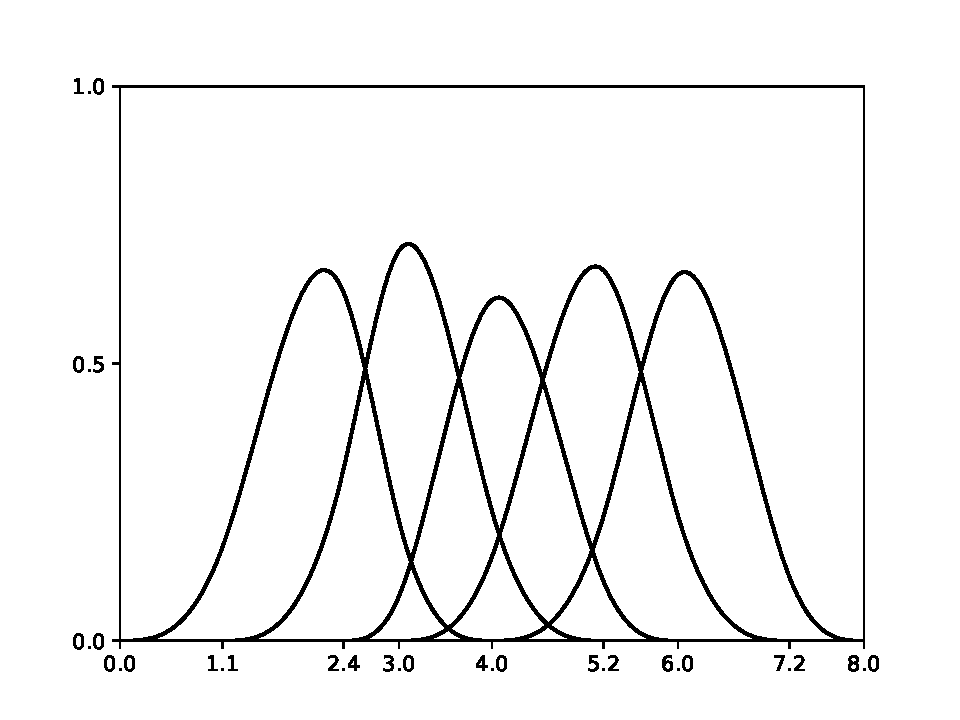
\includegraphics[width=0.6\linewidth]{3_bsplines/de_boor.pdf}
        \caption{Cubic B-splines on distinct knots computed with de Boor's algorithm without recursion. $n = 5$, with $\mathbf{t} = (0.0, 1.1, 2.4, 3, 4, 5.2, 6.0, 7.2, 8)$.\label{fig:spline_deboor}}
    \end{figure}
\end{solution}

\begin{exercise}
    Suppose that $d = 3$ and that the knot vector is
    \begin{equation*}
        \mathbf{t} = (0, 1, 2, 3, 4).
    \end{equation*}
    With this knot vector we can only associate one cubic B-spline, $B_{1,3}$.
    Therefore, if we want to compute $B_{1,3}(x)$ for some $x \in (0, 4)$, Algorithms~1 and~2 of Section~3.9 do not apply.
    Show, however, that by augmenting the knot vector to
    \begin{equation*}
        \hat{\mathbf{t}} = (0, 0, 0, 0, 1, 2, 3, 4, 4, 4, 4),
    \end{equation*}
    we can compute $B_{1,3}$ in the interval $(0, 4)$ using Algorithm~2.
\end{exercise}

\begin{solution}
    We begin by illustrating the indices of $\hat{\mathbf{t}}$ relative to $\mathbf{t}$.
    These are
    \begin{equation*}
        \hat{\mathbf{t}} = (t_{1-3}, t_{1-2}, t_{1-1}, t_1, t_2, t_3, t_4, t_5, t_{5+1}, t_{5+2}, t_{5+3}).
    \end{equation*}
    Then, for any $x \in (0, 4)$, we can find $\mu \in \{1, 2, 3, 4, 5\}$ such that $x \in [t_\mu, t_{\mu+1}]$.
    We can then compute $B_{1, 3}(x)$ by setting
    \begin{equation*}
        c_i^0 =
        \begin{cases}
            1, & i = 1 \\
            0, & \text{otherwise}
        \end{cases}
        \quad \text{for } i = \mu - 3, \ldots, \mu.
    \end{equation*}
    The algorithm then follows similarly, as for $r = 1, 2, 3$ and $i = \mu - 3 + r, \ldots, \mu$ we have
    \begin{equation*}
        c_i^r
        = \frac{t_{i+3-r+1} - x}{t_{i+3-r+1} - t_i} c_{i-1}^{r-1}
        + \frac{x - t_i}{t_{i+3-r+1} - t_{i}} c_{i}^{r-1}.
    \end{equation*}
    The result is then $B_{1, 3}(x) = c_{\mu}^3$.
    We are at most indexing $t_{i+3-r+1} = t_{\mu + 3}$, and atleast $t_i = t_{\mu - 3}$, so the algorithm is now well-defined for all points $x \in (0, 4)$.
\end{solution}
